% Компіляція: lualatex main.tex (двічі для коректного змісту й посилань)
\documentclass[12pt,a4paper]{article}

\usepackage{fontspec}
\usepackage{polyglossia}
\setdefaultlanguage{ukrainian}
\setmainfont{NewComputerModern10}
\setsansfont{Noto Sans}
\setmonofont{Noto Sans Mono}[
  Scale=0.85,
  ItalicFont={Noto Sans Mono},
  ItalicFeatures={FakeSlant=0.2}
]

\usepackage{
  amsmath,
  amssymb,
  array,
  booktabs,
  caption,
  enumitem,
  float,
  geometry,
  graphicx,
  microtype,
  titlesec,
  xcolor
}
\geometry{left=2cm,right=2cm,top=2cm,bottom=2cm}
\setlength{\parindent}{1.25cm}
\setlength{\parskip}{0pt}
\linespread{1.08}
\titleformat{\section}
  {\normalfont\fontsize{14}{16}\selectfont\bfseries}
  {\thesection}{0.6em}{}
\titleformat{\subsection}
  {\normalfont\fontsize{12}{14}\selectfont\bfseries}
  {\thesubsection}{0.6em}{}
\titlespacing*{\section}{0pt}{1.4em}{0.65em}
\titlespacing*{\subsection}{0pt}{1.1em}{0.45em}
\captionsetup{font=small,labelfont=bf,labelsep=endash}
\captionsetup[table]{position=bottom,skip=5pt}
\captionsetup[listing]{position=bottom,skip=0pt}

\usepackage[newfloat]{minted}
\SetupFloatingEnvironment{listing}{name=Лістинг}
\setminted{%
  fontsize=\footnotesize,
  linenos,
  breaklines,
  autogobble,
  frame=single,
  framesep=2mm,
  bgcolor=gray!5,
  tabsize=4
}

\usepackage[
  unicode,
  colorlinks=true,
  linkcolor=black,
  urlcolor=blue,
  pdftitle={ІО-41, Давидчук А. М., Методи та технології штучного інтелекту, Лабораторна робота №1},
  pdfauthor={Давидчук Артем},
  pdfsubject={Дослідження способів формування нечітких множин і операцій над ними}
]{hyperref}

% -----------------------------------------------------------------------------
% Дані, які найчастіше потрібно змінювати
% -----------------------------------------------------------------------------
\newcommand{\studentName}{Давидчук А. М.}
\newcommand{\studentGroup}{ІО-41}
\newcommand{\recordBook}{4106}
\newcommand{\teacherName}{Польшакова О. М.}
\newcommand{\reportYear}{2026}

\begin{document}

\pagenumbering{gobble}
\begin{titlepage}
  \begin{center}
    
\includegraphics[width=0.7\textwidth]{../../../../../templates/letterhead.png}
  \end{center}

  \begin{center}
    \large
    Національний технічний університет України\\
    «Київський політехнічний інститут імені Ігоря Сікорського»\\[1em]
    Факультет інформатики та обчислювальної техніки\\
    Кафедра обчислювальної техніки
  \end{center}

  \vfill

  \begin{center}
    \textbf{\LARGE Методи та технології штучного інтелекту}\\[2em]
    \textbf{\Large Лабораторна робота №1}\\[0.7em]
    \parbox{0.9\textwidth}{\centering
      «Дослідження способів формування нечітких множин і операцій над ними»}
  \end{center}

  \vfill

  \begin{flushright}
    \begin{minipage}{0.48\textwidth}
      Виконав: студент 3 курсу ФІОТ,\\
      групи \studentGroup\\
      \textit{\studentName}\\
      Залікова книжка № \recordBook\\[1em]
      Перевірив: \textit{\teacherName}
    \end{minipage}
  \end{flushright}

  \vfill

  \begin{center}Київ --- \reportYear\end{center}
\end{titlepage}
\pagenumbering{arabic}

\section{Тема та мета роботи}

\noindent
\textbf{Тема:} дослідження способів формування нечітких множин і операцій над
ними.

\medskip

\noindent
\textbf{Мета:} побудувати нечіткі множини з використанням різних типів
функцій приналежності; виконати найбільш поширені логічні операції над
нечіткими множинами.

\section{Теоретичні відомості}

Нечітка множина $A$ на універсальній множині $X$ задається функцією
приналежності $\mu_A(x)\colon X\to[0;1]$. Значення $\mu_A(x)$ характеризує
ступінь, із яким елемент $x$ належить множині $A$. На відміну від чіткої
множини, проміжні значення між 0 та 1 дозволяють описувати часткову
приналежність.

У роботі досліджуються такі типи функцій приналежності:

\begin{itemize}[leftmargin=*,itemsep=0.25em]
  \item трикутна $\operatorname{trimf}(x; a,b,c)$ та трапецієподібна
    $\operatorname{trapmf}(x; a,b,c,d)$;
  \item проста й двостороння гаусові $\operatorname{gaussmf}$ та
    $\operatorname{gauss2mf}$;
  \item узагальнена дзвоноподібна $\operatorname{gbellmf}$;
  \item сигмоїдальні $\operatorname{sigmf}$, $\operatorname{dsigmf}$ і
    $\operatorname{psigmf}$;
  \item поліноміальні Z-, PI- та S-функції: $\operatorname{zmf}$,
    $\operatorname{pimf}$ і $\operatorname{smf}$.
\end{itemize}

Наприклад, трикутна функція приналежності має вигляд
\begin{equation}
  \mu(x)=
  \begin{cases}
    0, & x\le a,\\
    \dfrac{x-a}{b-a}, & a<x\le b,\\
    \dfrac{c-x}{c-b}, & b<x<c,\\
    0, & x\ge c,
  \end{cases}
  \qquad a\le b\le c.
  \label{eq:trimf}
\end{equation}
а проста гаусова функція задається формулою
\begin{equation}
  \mu(x)=\exp\!\left(-\frac{(x-c)^2}{2\sigma^2}\right).
  \label{eq:gaussmf}
\end{equation}
Для двох нечітких множин $A$ і $B$ мінімаксна інтерпретація перетину та
об'єднання задається відповідно як
\begin{equation}
  \begin{aligned}
    \mu_{A\cap B}(x)&=\min\!\bigl(\mu_A(x),\mu_B(x)\bigr),\\
    \mu_{A\cup B}(x)&=\max\!\bigl(\mu_A(x),\mu_B(x)\bigr).
  \end{aligned}
  \label{eq:minmax}
\end{equation}
В імовірнісній інтерпретації використовують алгебраїчний добуток і
алгебраїчну суму:
\begin{equation}
  \begin{aligned}
    \mu_{A\cap B}(x)&=\mu_A(x)\mu_B(x),\\
    \mu_{A\cup B}(x)&=\mu_A(x)+\mu_B(x)-\mu_A(x)\mu_B(x).
  \end{aligned}
  \label{eq:probabilistic}
\end{equation}
Доповнення нечіткої множини визначається формулою
\begin{equation}
  \mu_{\overline A}(x)=1-\mu_A(x).
  \label{eq:complement}
\end{equation}

\section{Хід роботи}

Для програмної реалізації використовується мова Python, бібліотека
\texttt{scikit-fuzzy} (імпортується як \texttt{skfuzzy}) та засоби
\texttt{NumPy} і \texttt{Matplotlib}. Загальний порядок виконання роботи був
таким:

  \begin{enumerate}[leftmargin=*,itemsep=0.25em]
    \item Підготувати програмне середовище та під'єднати потрібні бібліотеки.
    \item Сформувати універсальну множину і побудувати трикутну та
      трапецієподібну функції приналежності.
    \item Побудувати просту гаусову функцію і три варіанти двосторонньої
      гаусової функції з різними параметрами.
    \item Побудувати узагальнену дзвоноподібну, сигмоїдальні та поліноміальні
      функції приналежності.
    \item Для двох нечітких множин виконати операції перетину й об'єднання в
      мінімаксній та імовірнісній інтерпретаціях.
    \item Побудувати доповнення однієї з нечітких множин.
    \item Зберегти код, параметри й графіки та проаналізувати результати.
  \end{enumerate}

\section{Результати}

\subsection{Підготовка програмного середовища}

Роботу виконано в Jupyter Notebook у локальному віртуальному середовищі
\texttt{.venv}. Використані версії програмних засобів наведено в
табл.~\ref{tab:environment}. Бібліотеки встановлено за допомогою менеджера
пакетів \texttt{pip}; точні залежності зафіксовано у файлі
\texttt{requirements.txt}.

\begin{table}[H]
  \centering
  \renewcommand{\arraystretch}{1.18}
  \begin{tabular}{|l|l|}
    \hline
    \textbf{Складова} & \textbf{Версія} \\
    \hline
    Python & 3.14.7 \\ \hline
    NumPy & 2.5.3 \\ \hline
    SciPy & 1.18.1 \\ \hline
    Matplotlib & 3.11.2 \\ \hline
    scikit-fuzzy & 0.5.0 \\ \hline
  \end{tabular}
  \caption{Параметри програмного середовища}
  \label{tab:environment}
\end{table}

Для всіх побудов використано спільну універсальну множину
\(X=[-10;10]\) із кроком \(h=0{,}02\), що містить 1001 точку. Така
дискретизація забезпечує плавне відображення кривих і дозволяє виконувати
поточкові операції над масивами однакової довжини.

\begin{listing}[H]
\begin{minted}{python}
from pathlib import Path
import numpy as np
import matplotlib.pyplot as plt
import skfuzzy as fuzz

FIGURES_DIR = Path("figures")
FIGURES_DIR.mkdir(exist_ok=True)
x = np.arange(-10.0, 10.0 + 0.02 / 2, 0.02)
\end{minted}
\caption{Підготовка середовища та універсальної множини}
\end{listing}

\subsection{Трикутна та трапецієподібна функції приналежності}

Трикутну функцію побудовано з параметрами \([-8,-3,2]\), а
трапецієподібну --- з параметрами \([-1,2,5,8]\). Реалізацію наведено в
лістингу~\ref{lst:tri-trap}, результат --- на рис.~\ref{fig:tri-trap}.

\begin{listing}[H]
\begin{minted}{python}
mu_tri = fuzz.trimf(x, [-8, -3, 2])
mu_trap = fuzz.trapmf(x, [-1, 2, 5, 8])
\end{minted}
\caption{Побудова трикутної та трапецієподібної функцій}
\label{lst:tri-trap}
\end{listing}

\begin{figure}[H]
  \centering
  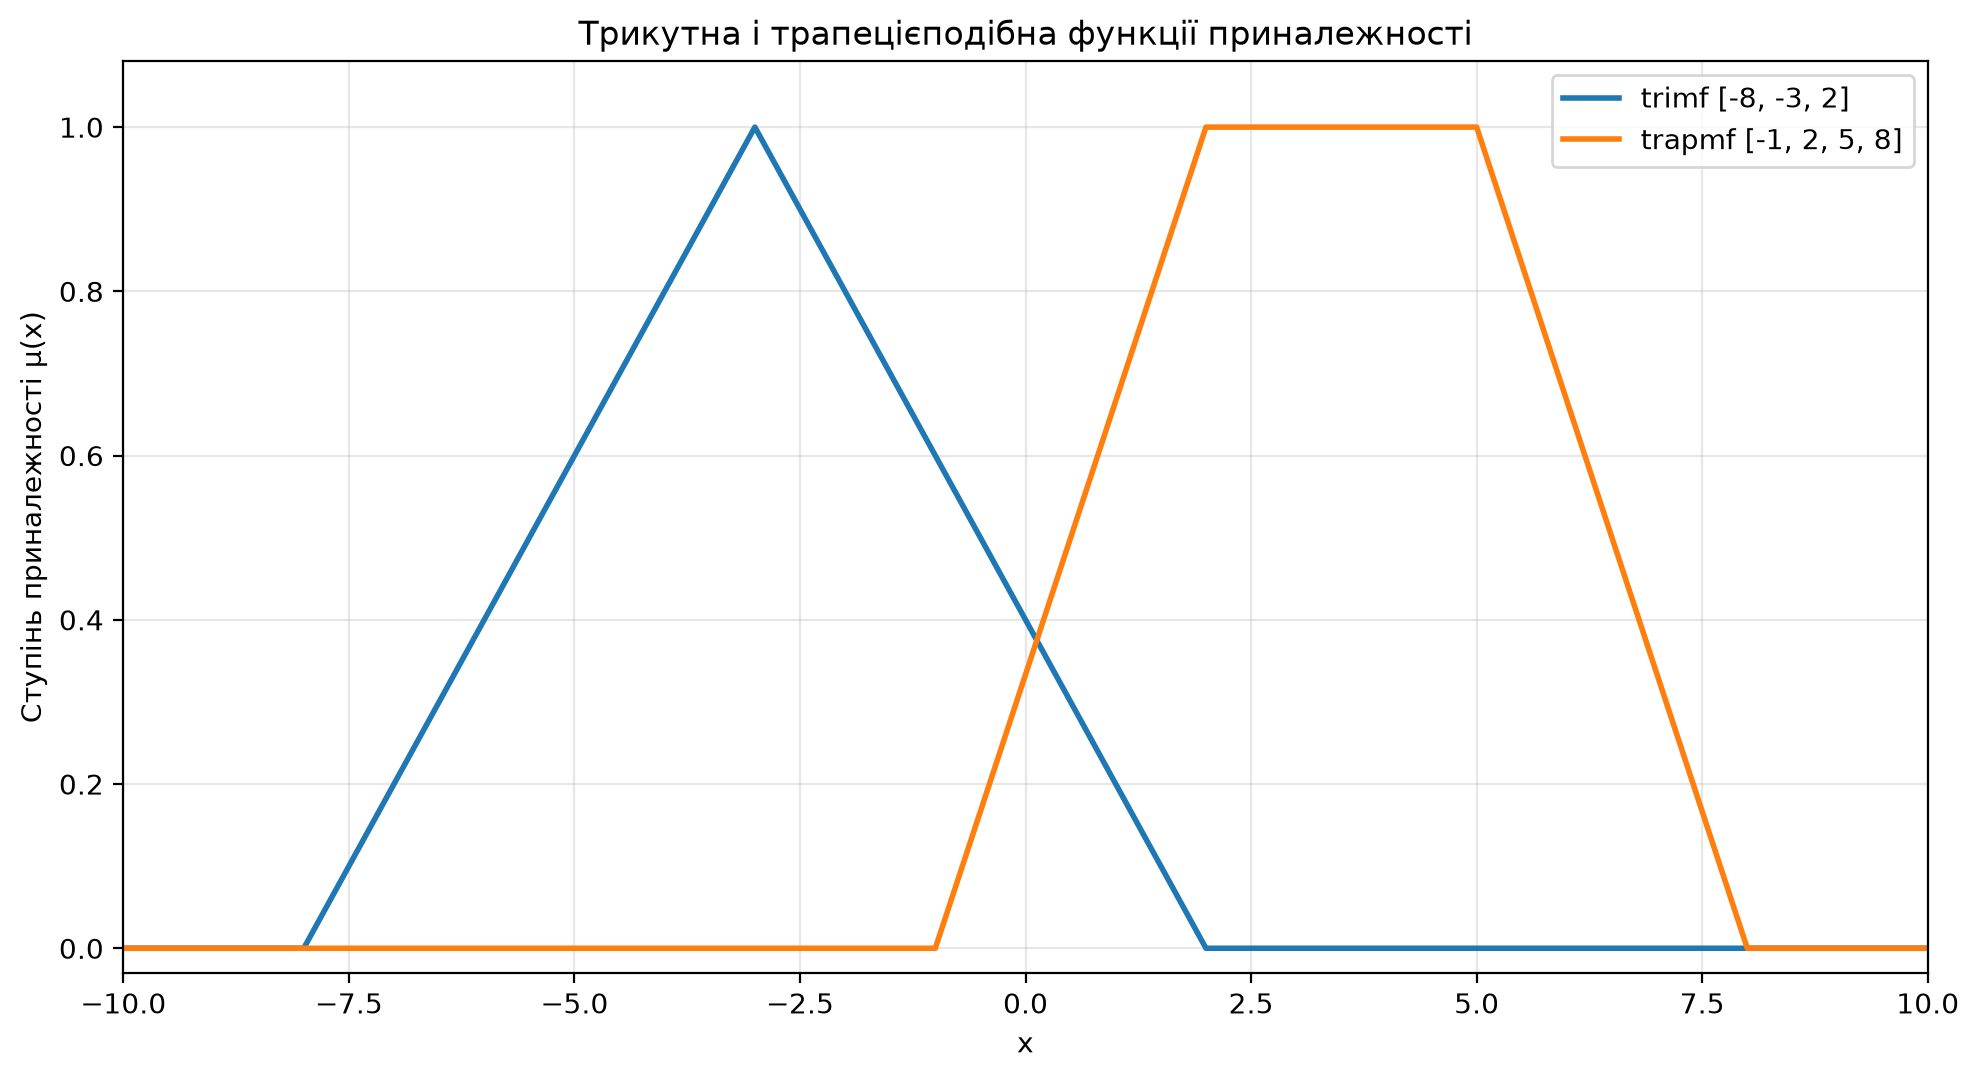
\includegraphics[width=\textwidth,height=0.42\textheight,keepaspectratio]{../src/figures/01_tri_trap.png}
  \caption{Трикутна та трапецієподібна функції приналежності}
  \label{fig:tri-trap}
\end{figure}

\noindent
\textbf{Спостереження:}
трикутна функція досягає одиниці лише у вершині \(x=-3\), тоді як
трапецієподібна має плато повної приналежності на відрізку \([2;5]\).
Крайні параметри задають носій, а внутрішні --- положення вершини або межі
плато.

\subsection{Проста та двостороння гаусові функції приналежності}

Параметри простої та трьох двосторонніх гаусових функцій наведено в
табл.~\ref{tab:gaussian}. Для \texttt{gauss2mf} між двома центрами значення
функції дорівнює одиниці.

\begin{table}[H]
  \centering
  \renewcommand{\arraystretch}{1.18}
  \begin{tabular}{|l|r|r|r|r|}
    \hline
    \textbf{Функція} & \(c_1\) & \(\sigma_1\) & \(c_2\) & \(\sigma_2\) \\
    \hline
    \texttt{gaussmf}  & 0  & 2{,}0 & --- & --- \\ \hline
    \texttt{gauss2mf} №1 & -6 & 1{,}0 & -2 & 1{,}0 \\ \hline
    \texttt{gauss2mf} №2 & -5 & 1{,}5 &  2 & 0{,}8 \\ \hline
    \texttt{gauss2mf} №3 & -3 & 0{,}8 &  4 & 2{,}0 \\ \hline
  \end{tabular}
  \caption{Параметри гаусових функцій}
  \label{tab:gaussian}
\end{table}

\begin{listing}[H]
\begin{minted}{python}
mu_gauss = fuzz.gaussmf(x, mean=0, sigma=2)
for p in GAUSS2:
    mu_gauss2 = fuzz.gauss2mf(x, **p)
\end{minted}
\caption{Побудова гаусових функцій}
\end{listing}

\begin{figure}[H]
  \centering
  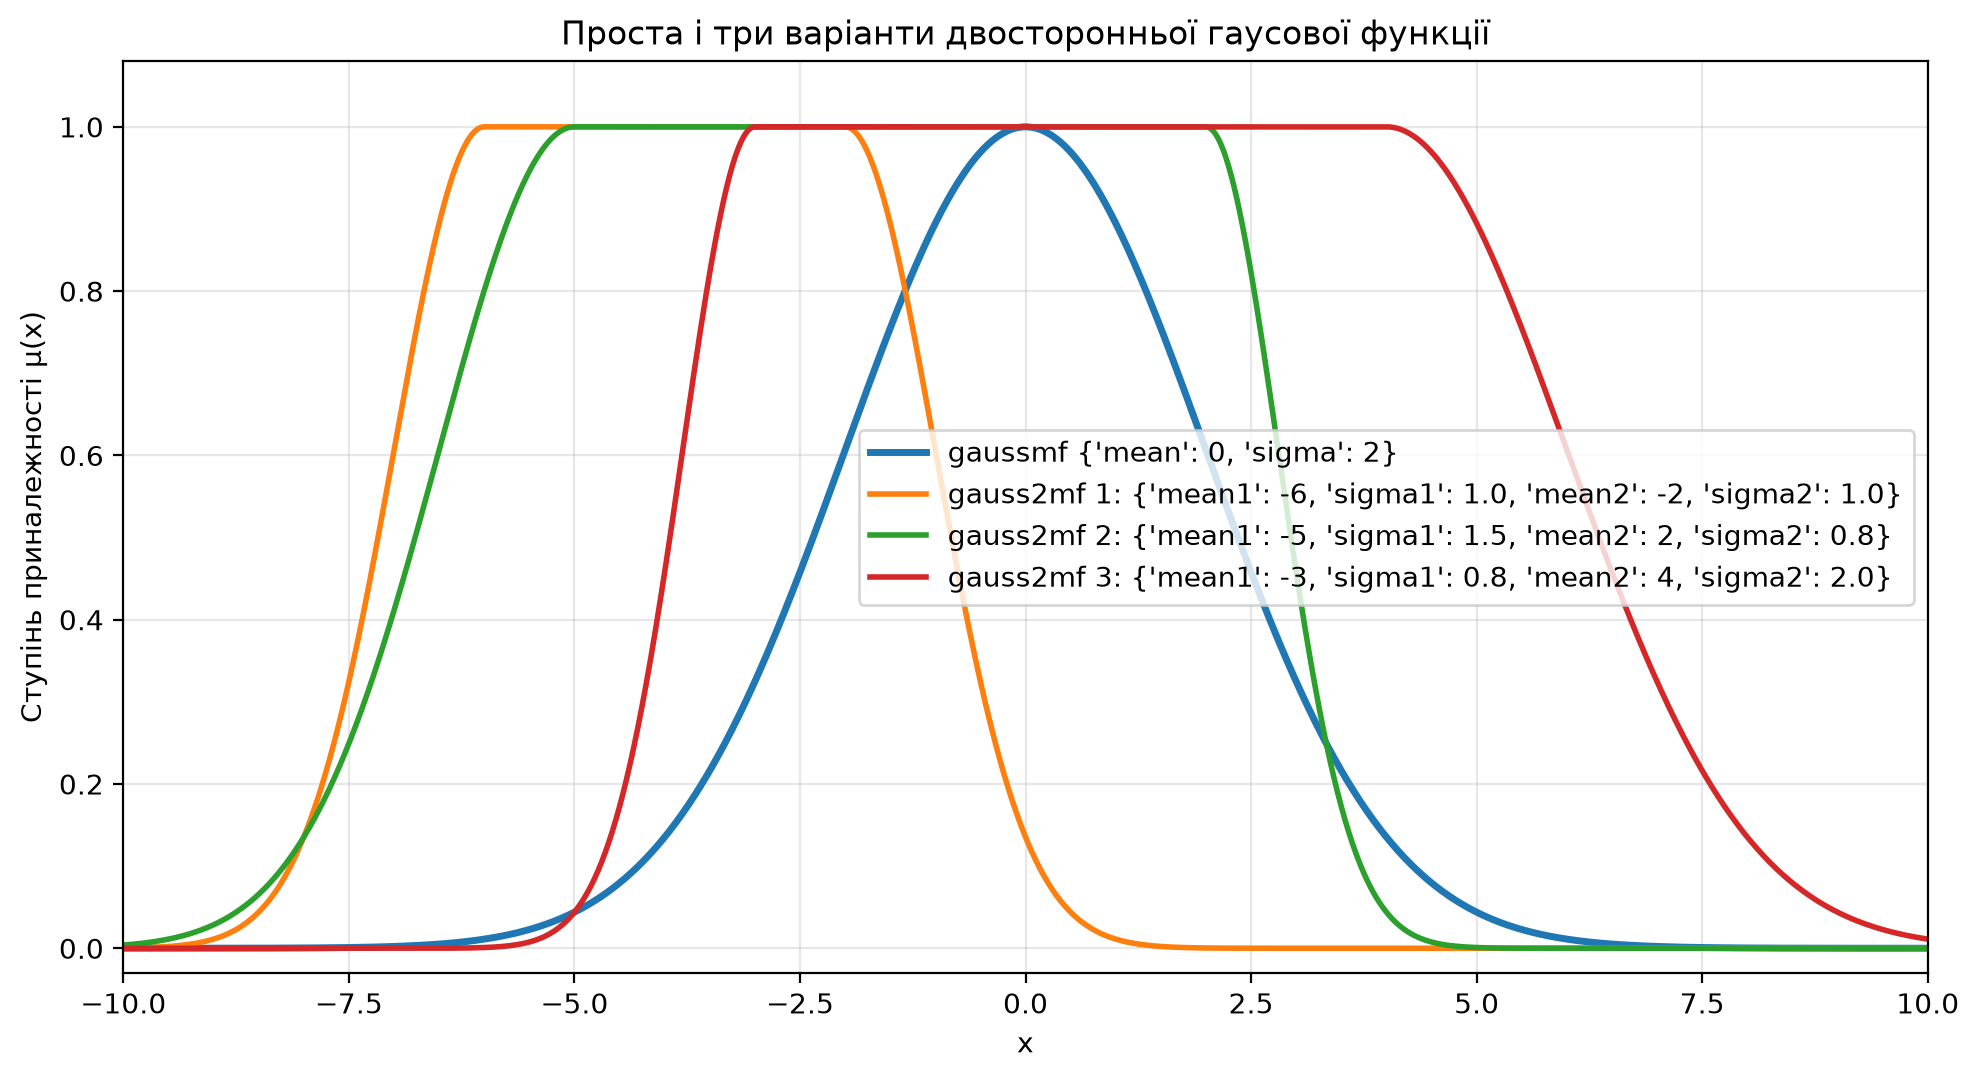
\includegraphics[width=\textwidth,height=0.42\textheight,keepaspectratio]{../src/figures/02_gaussian.png}
  \caption{Проста та три двосторонні гаусові функції приналежності}
  \label{fig:gaussian}
\end{figure}

\noindent
\textbf{Спостереження:}
центри переміщують межі плато вздовж осі \(x\), а значення \(\sigma\)
визначають пологість відповідного схилу. У другому і третьому варіантах
різні \(\sigma_1\) та \(\sigma_2\) утворюють асиметричні переходи.

\subsection{Функція приналежності «узагальнений дзвін»}

Використано параметри \(a=2{,}5\), \(b=3\), \(c=0\).

\begin{listing}[H]
\begin{minted}{python}
mu_gbell = fuzz.gbellmf(x, a=2.5, b=3, c=0)
\end{minted}
\caption{Побудова узагальненої дзвоноподібної функції}
\end{listing}

\begin{figure}[H]
  \centering
  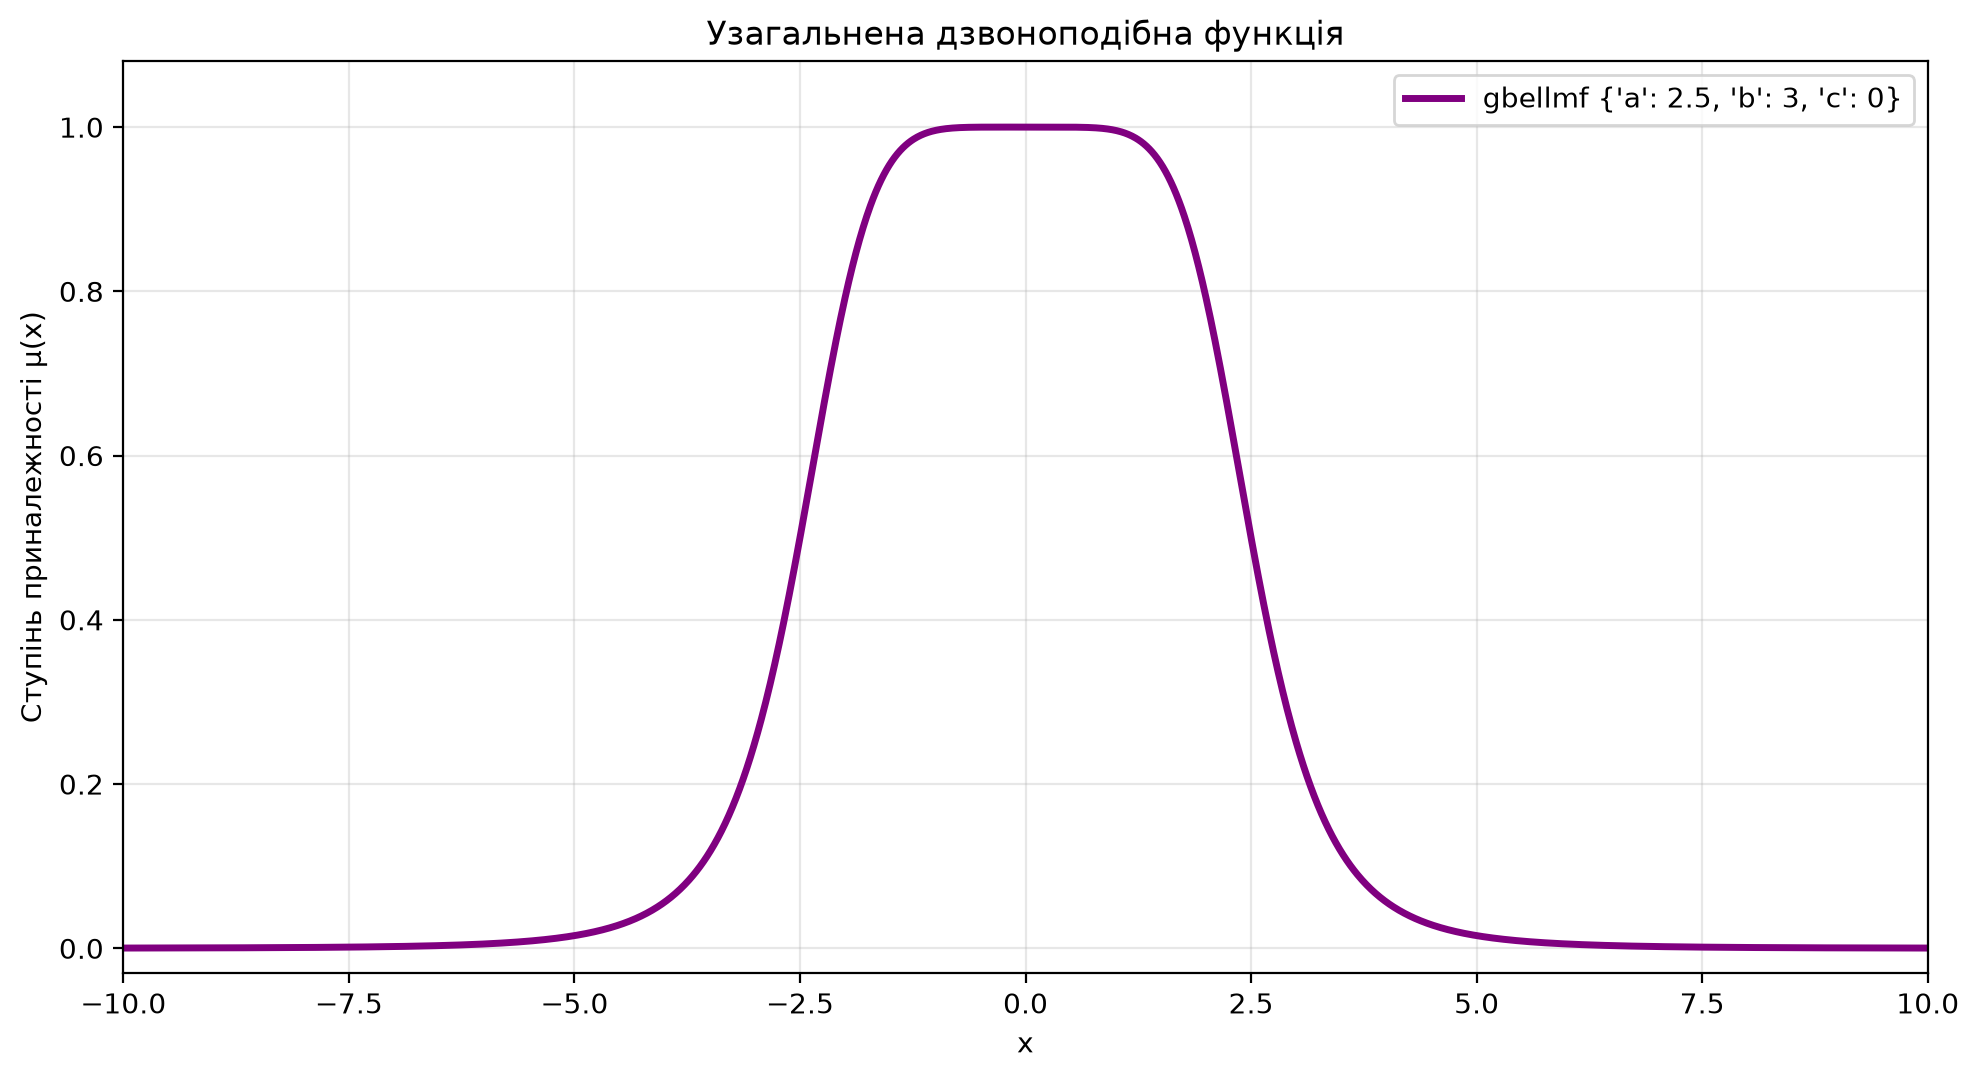
\includegraphics[width=\textwidth,height=0.42\textheight,keepaspectratio]{../src/figures/03_gbell.png}
  \caption{Узагальнена дзвоноподібна функція приналежності}
  \label{fig:gbell}
\end{figure}

\noindent
\textbf{Спостереження:}
параметр \(c\) задає центр кривої, \(a\) --- її ширину, а \(b\) ---
крутизну переходів. За вибраних параметрів отримано симетричну відносно
нуля криву з плавною вершиною та доволі крутими схилами.

\subsection{Сигмоїдальні функції приналежності}

З урахуванням сигнатур \texttt{scikit-fuzzy 0.5.0} задано такі параметри:
\texttt{sigmf}: \(b=-1\), \(c=1{,}5\); \texttt{dsigmf}:
\(b_1=-4\), \(c_1=1{,}8\), \(b_2=4\), \(c_2=1{,}8\);
\texttt{psigmf}: \(b_1=-5\), \(c_1=1{,}2\), \(b_2=3\),
\(c_2=-2{,}5\).

\begin{listing}[H]
\begin{minted}{python}
mu_sig  = fuzz.sigmf(x, **SIG)
mu_dsig = fuzz.dsigmf(x, **DSIG)
mu_psig = fuzz.psigmf(x, **PSIG)
\end{minted}
\caption{Побудова сигмоїдальних функцій}
\end{listing}

\begin{figure}[H]
  \centering
  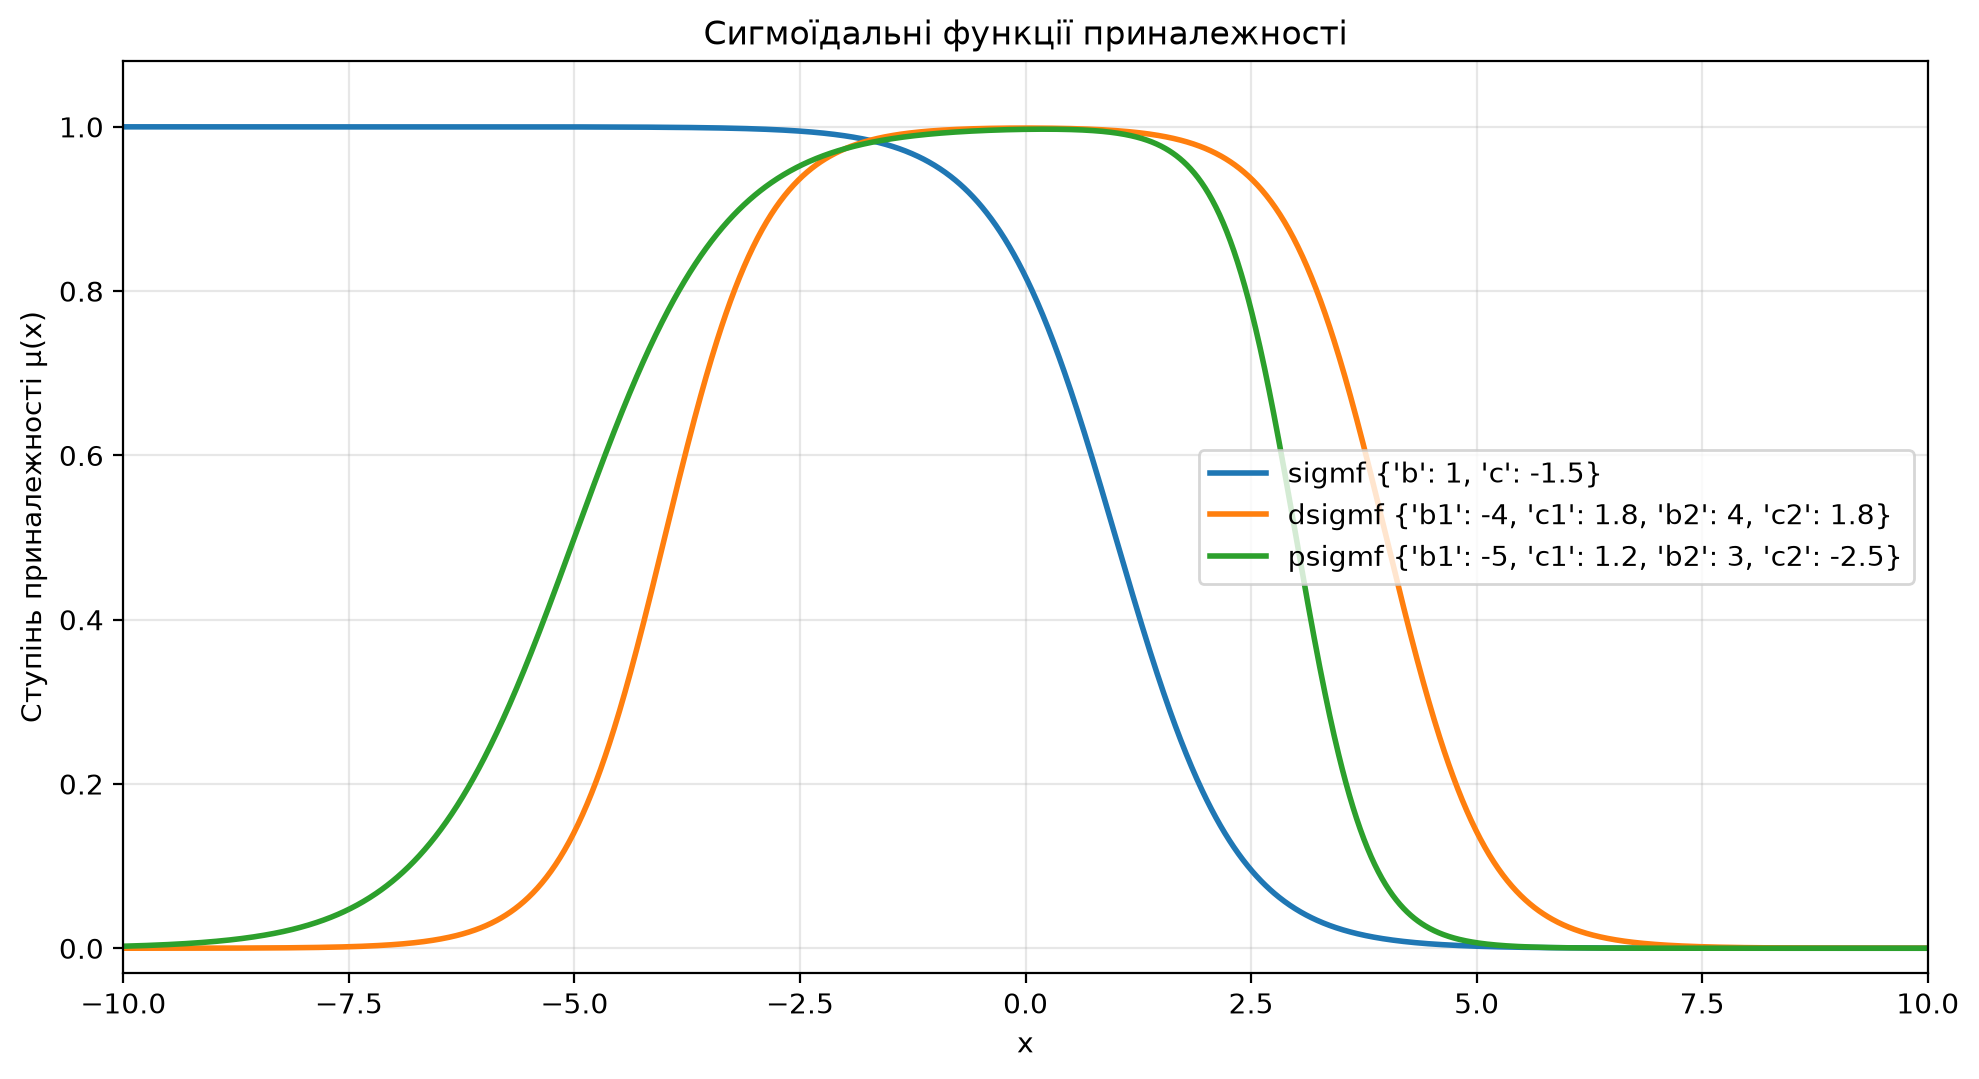
\includegraphics[width=\textwidth,height=0.42\textheight,keepaspectratio]{../src/figures/04_sigmoid.png}
  \caption{Сигмоїдальні функції приналежності}
  \label{fig:sigmoid}
\end{figure}

\noindent
\textbf{Спостереження:}
\texttt{sigmf} формує односторонній зростаючий перехід. Різниця двох
сигмоїд \texttt{dsigmf} утворює двосторонню область високої приналежності.
Для \texttt{psigmf} протилежні знаки нахилів формують замкнену область, а
нерівні модулі \(c_1\) та \(c_2\) роблять її асиметричною.

\subsection{Поліноміальні функції приналежності}

Для Z-функції використано \(a=-6\), \(b=0\); для PI-функції ---
\(a=-7\), \(b=-3\), \(c=2\), \(d=7\); для S-функції --- \(a=0\),
\(b=7\).

\begin{listing}[H]
\begin{minted}{python}
mu_z  = fuzz.zmf(x, a=-6, b=0)
mu_pi = fuzz.pimf(x, a=-7, b=-3, c=2, d=7)
mu_s  = fuzz.smf(x, a=0, b=7)
\end{minted}
\caption{Побудова поліноміальних функцій}
\end{listing}

\begin{figure}[H]
  \centering
  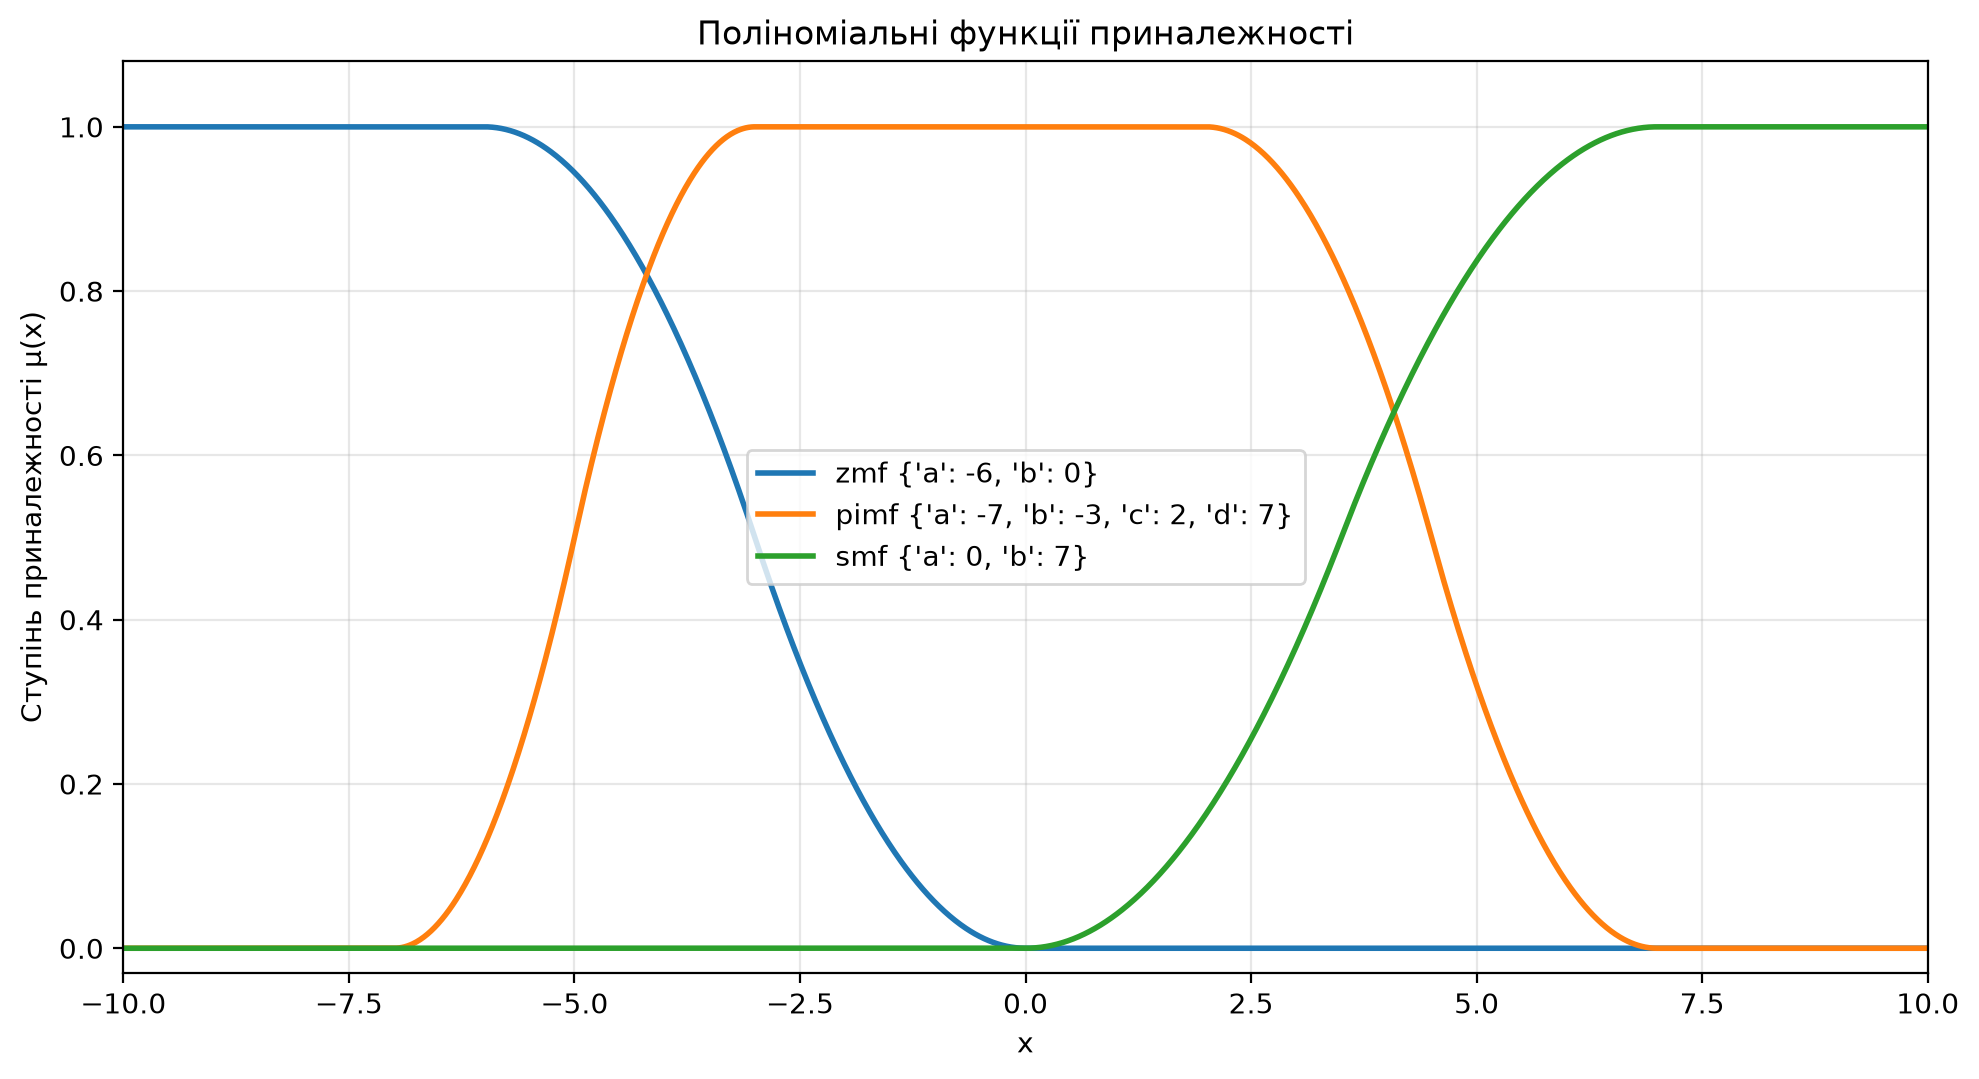
\includegraphics[width=\textwidth,height=0.42\textheight,keepaspectratio]{../src/figures/05_polynomial.png}
  \caption{Поліноміальні Z-, PI- та S-функції приналежності}
  \label{fig:polynomial}
\end{figure}

\noindent
\textbf{Спостереження:}
у Z-функції повна приналежність спостерігається при \(x\leq-6\), часткова
--- на \((-6;0)\), нульова --- при \(x\geq0\). Для S-функції відповідні
ділянки розташовані у зворотному порядку. PI-функція має нульові зовнішні
ділянки, переходи на \((-7;-3)\) та \((2;7)\), а також плато одиничної
приналежності \([-3;2]\).

\subsection{Мінімаксна інтерпретація логічних операторів}

Для операцій вибрано дві гаусові нечіткі множини на спільному універсумі.
Для множини \(A\) центр дорівнює \(-2{,}5\), а \(\sigma_A=2{,}0\); для
множини \(B\) центр дорівнює \(2{,}5\), а \(\sigma_B=2{,}5\).

\begin{listing}[H]
\begin{minted}{python}
mu_a = fuzz.gaussmf(x, mean=-2.5, sigma=2.0)
mu_b = fuzz.gaussmf(x, mean= 2.5, sigma=2.5)
min_intersection = np.fmin(mu_a, mu_b)
max_union = np.fmax(mu_a, mu_b)
\end{minted}
\caption{Мінімаксні операції над нечіткими множинами}
\end{listing}

\begin{figure}[H]
  \centering
  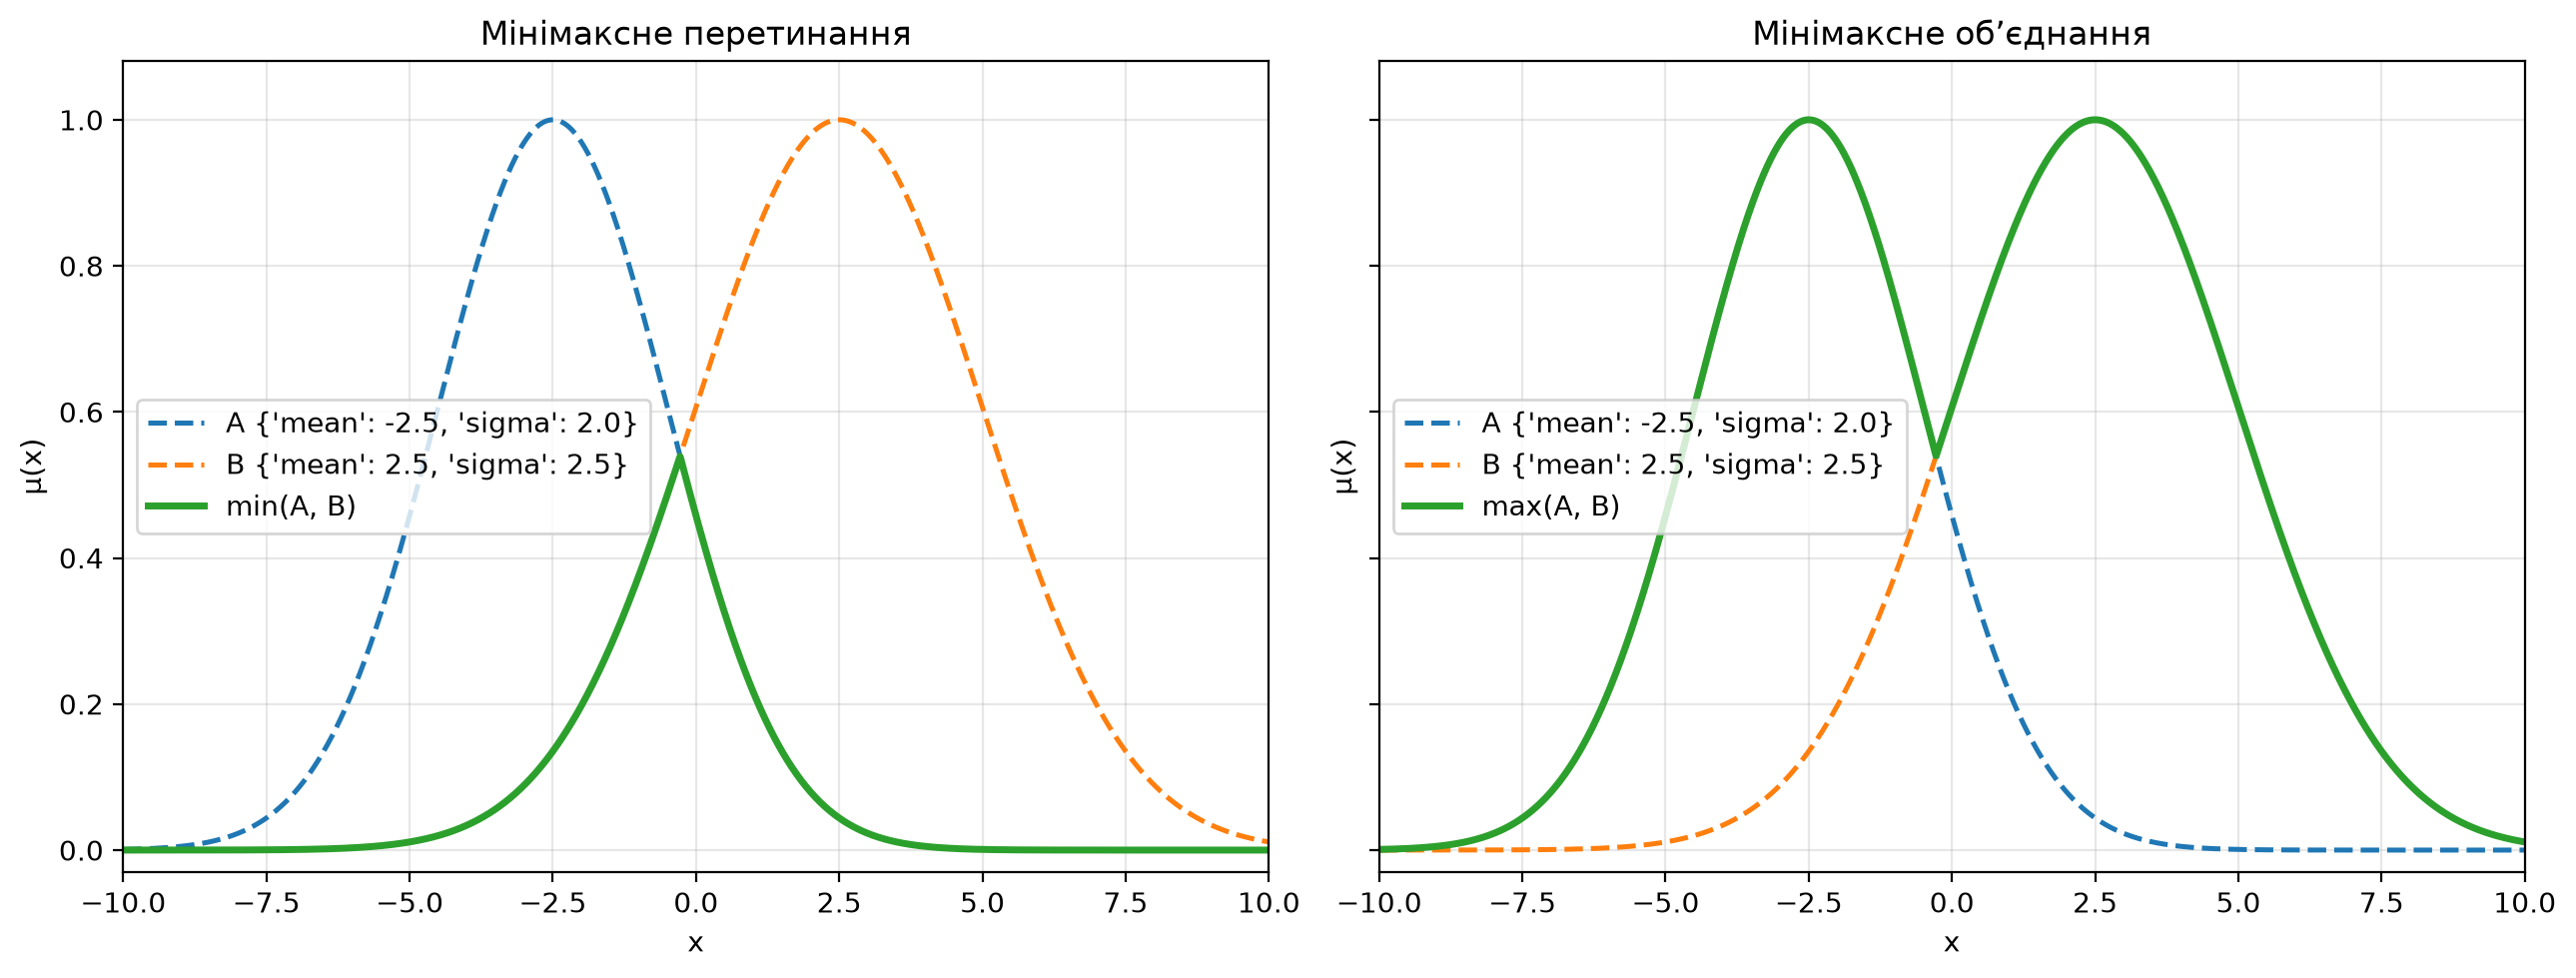
\includegraphics[width=\textwidth,height=0.42\textheight,keepaspectratio]{../src/figures/06_minmax.png}
  \caption{Мінімаксні перетин та об'єднання нечітких множин}
  \label{fig:minmax}
\end{figure}

\noindent
\textbf{Спостереження:}
перетин у кожній точці збігається з нижчою з двох початкових кривих, а
об'єднання --- з вищою. У зоні переважання \(A\) об'єднання повторює
\(A\), а перетин --- \(B\); після точки перетину ролі кривих змінюються.

\subsection{Імовірнісна інтерпретація логічних операторів}

Для тих самих множин \(A\) і \(B\) обчислено алгебраїчний добуток та
алгебраїчну суму. На рис.~\ref{fig:probability} кожний результат показано
разом із двома вихідними кривими, а на рис.~\ref{fig:comparison} наведено
порівняння з мінімаксними операціями.

\begin{listing}[H]
\begin{minted}{python}
algebraic_product = mu_a * mu_b
algebraic_sum = mu_a + mu_b - mu_a * mu_b
\end{minted}
\caption{Імовірнісні операції над нечіткими множинами}
\end{listing}

\begin{figure}[H]
  \centering
  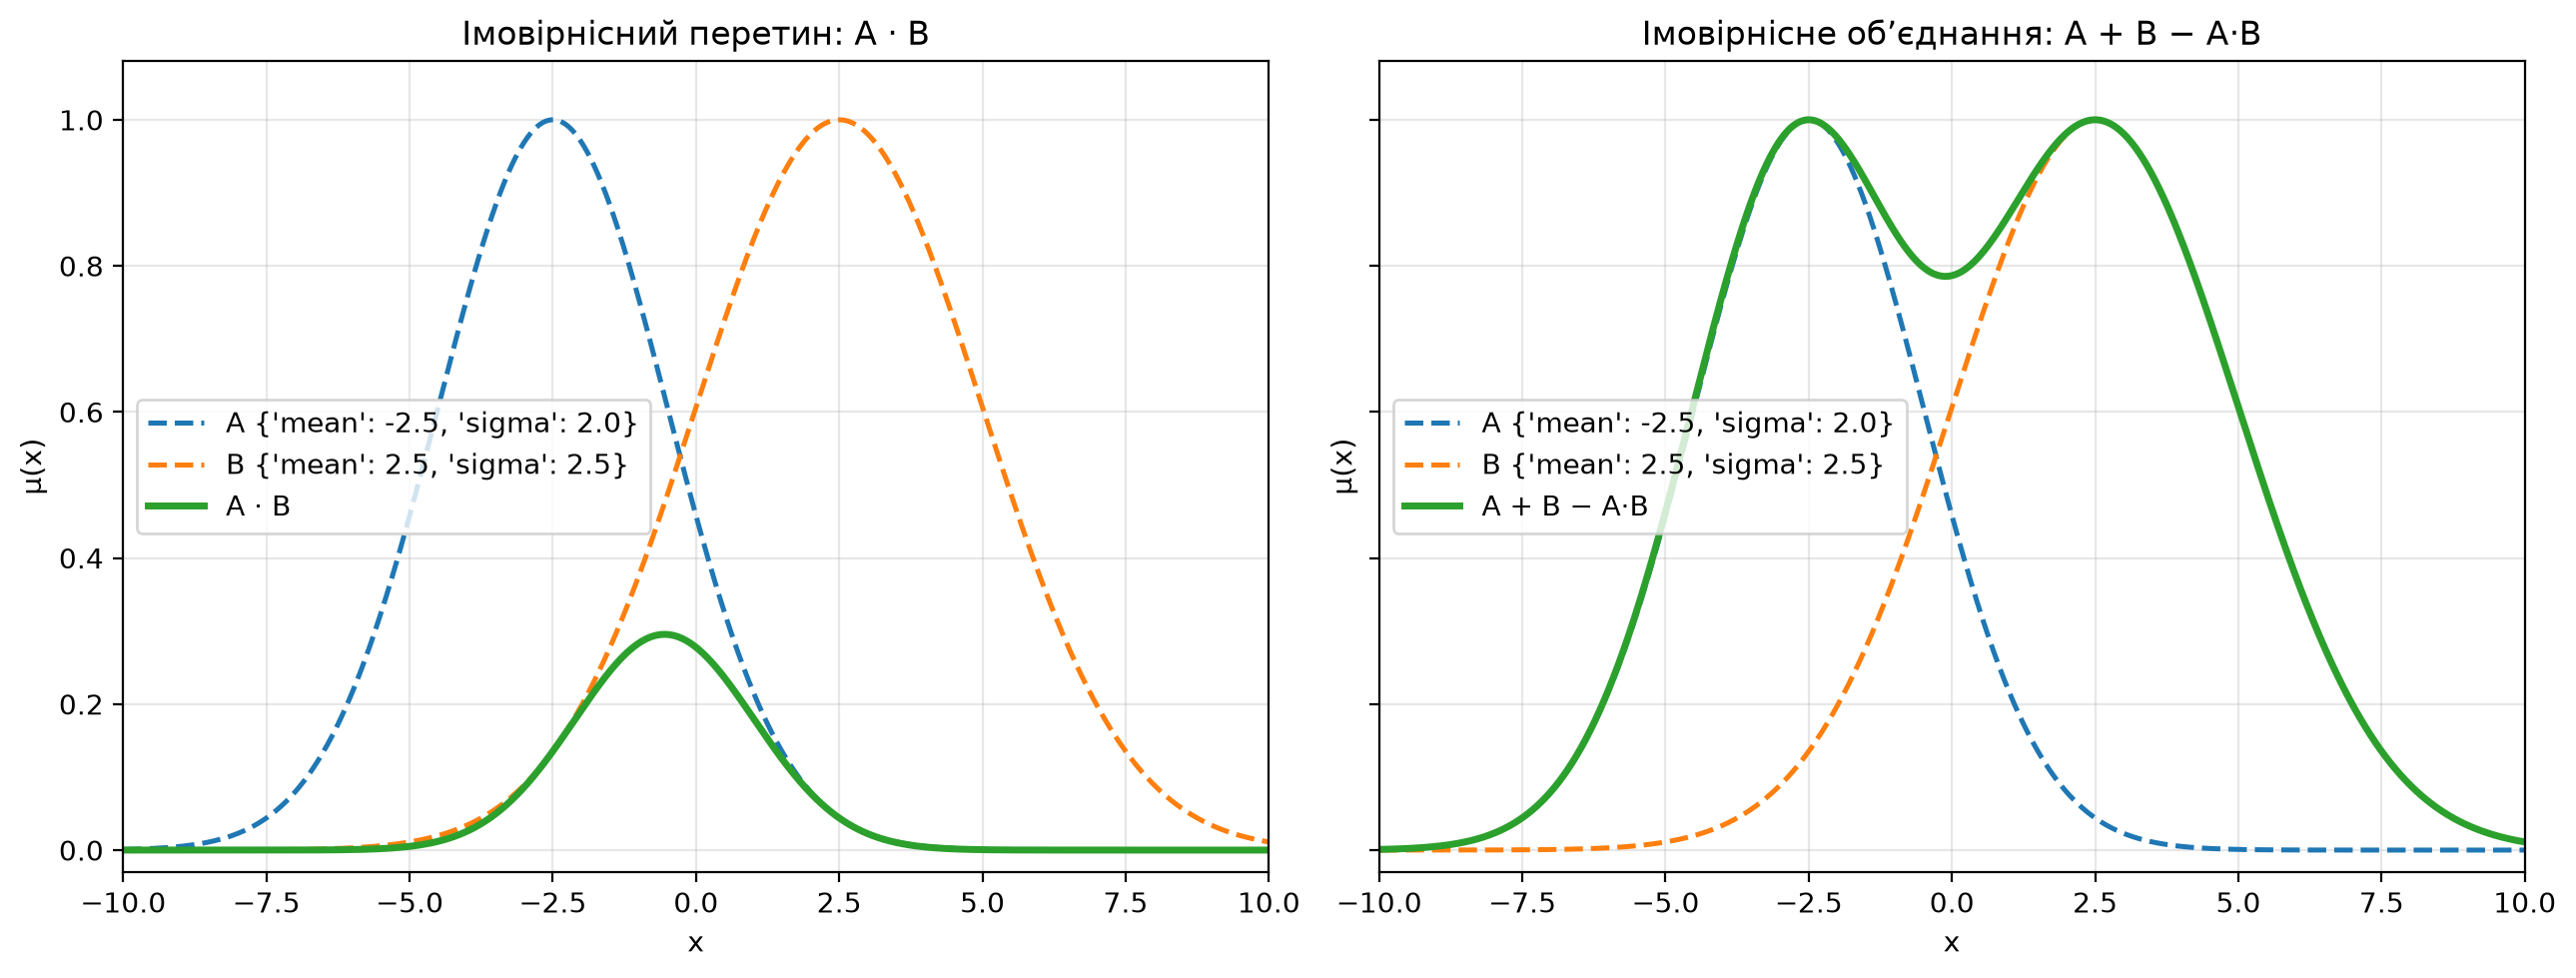
\includegraphics[width=\textwidth,height=0.42\textheight,keepaspectratio]{../src/figures/07_probabilistic.png}
  \caption{Імовірнісні перетин та об'єднання разом із множинами \(A\) і \(B\)}
  \label{fig:probability}
\end{figure}

\begin{figure}[H]
  \centering
  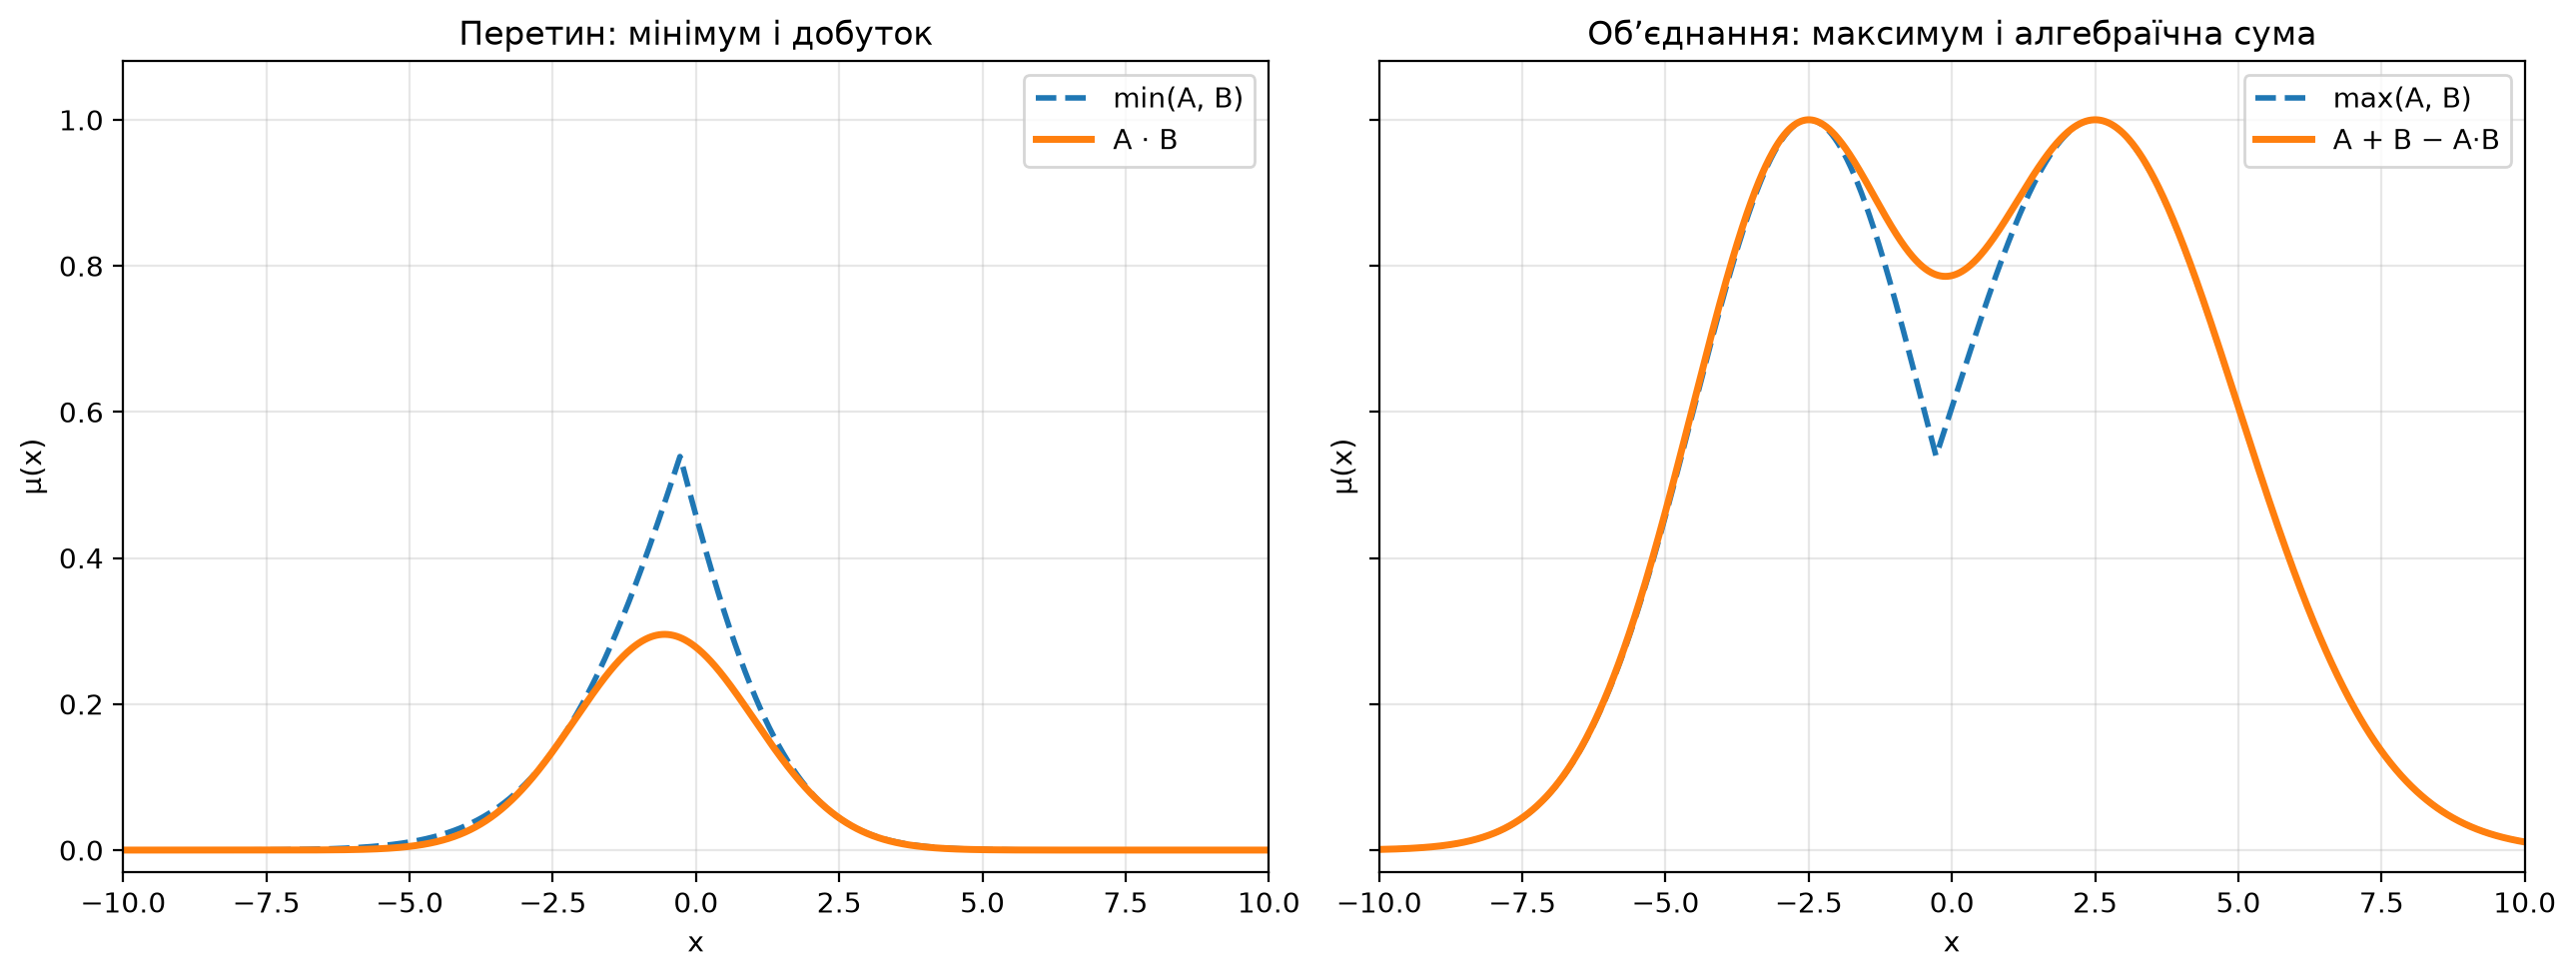
\includegraphics[width=\textwidth,height=0.42\textheight,keepaspectratio]{../src/figures/08_probabilistic_comparison.png}
  \caption{Порівняння імовірнісної та мінімаксної інтерпретацій}
  \label{fig:comparison}
\end{figure}

\noindent
\textbf{Спостереження:}
числова перевірка підтвердила, що \(\mu_A\mu_B\leq
\min(\mu_A,\mu_B)\), тому алгебраїчний добуток дає суворіший перетин.
Водночас \(\mu_A+\mu_B-\mu_A\mu_B\geq\max(\mu_A,\mu_B)\), тобто
алгебраїчна сума дає м'якше об'єднання. Обидві нерівності виконуються для
всіх 1001 точок універсуму.

\subsection{Доповнення нечіткої множини}

Доповнення побудовано для множини \(A\). Початкове судження сформульовано як
«значення \(x\) є близьким до \(-2{,}5\)», а його заперечення --- «значення
\(x\) не є близьким до \(-2{,}5\)». Додатково на графіку показано
\(\alpha\)-зріз для \(\alpha=0{,}5\).

\begin{listing}[H]
\begin{minted}{python}
mu_not_a = 1 - mu_a
alpha_mask = mu_a >= 0.5
assert np.allclose(mu_a + mu_not_a, 1)
\end{minted}
\caption{Побудова й перевірка доповнення}
\end{listing}

\begin{figure}[H]
  \centering
  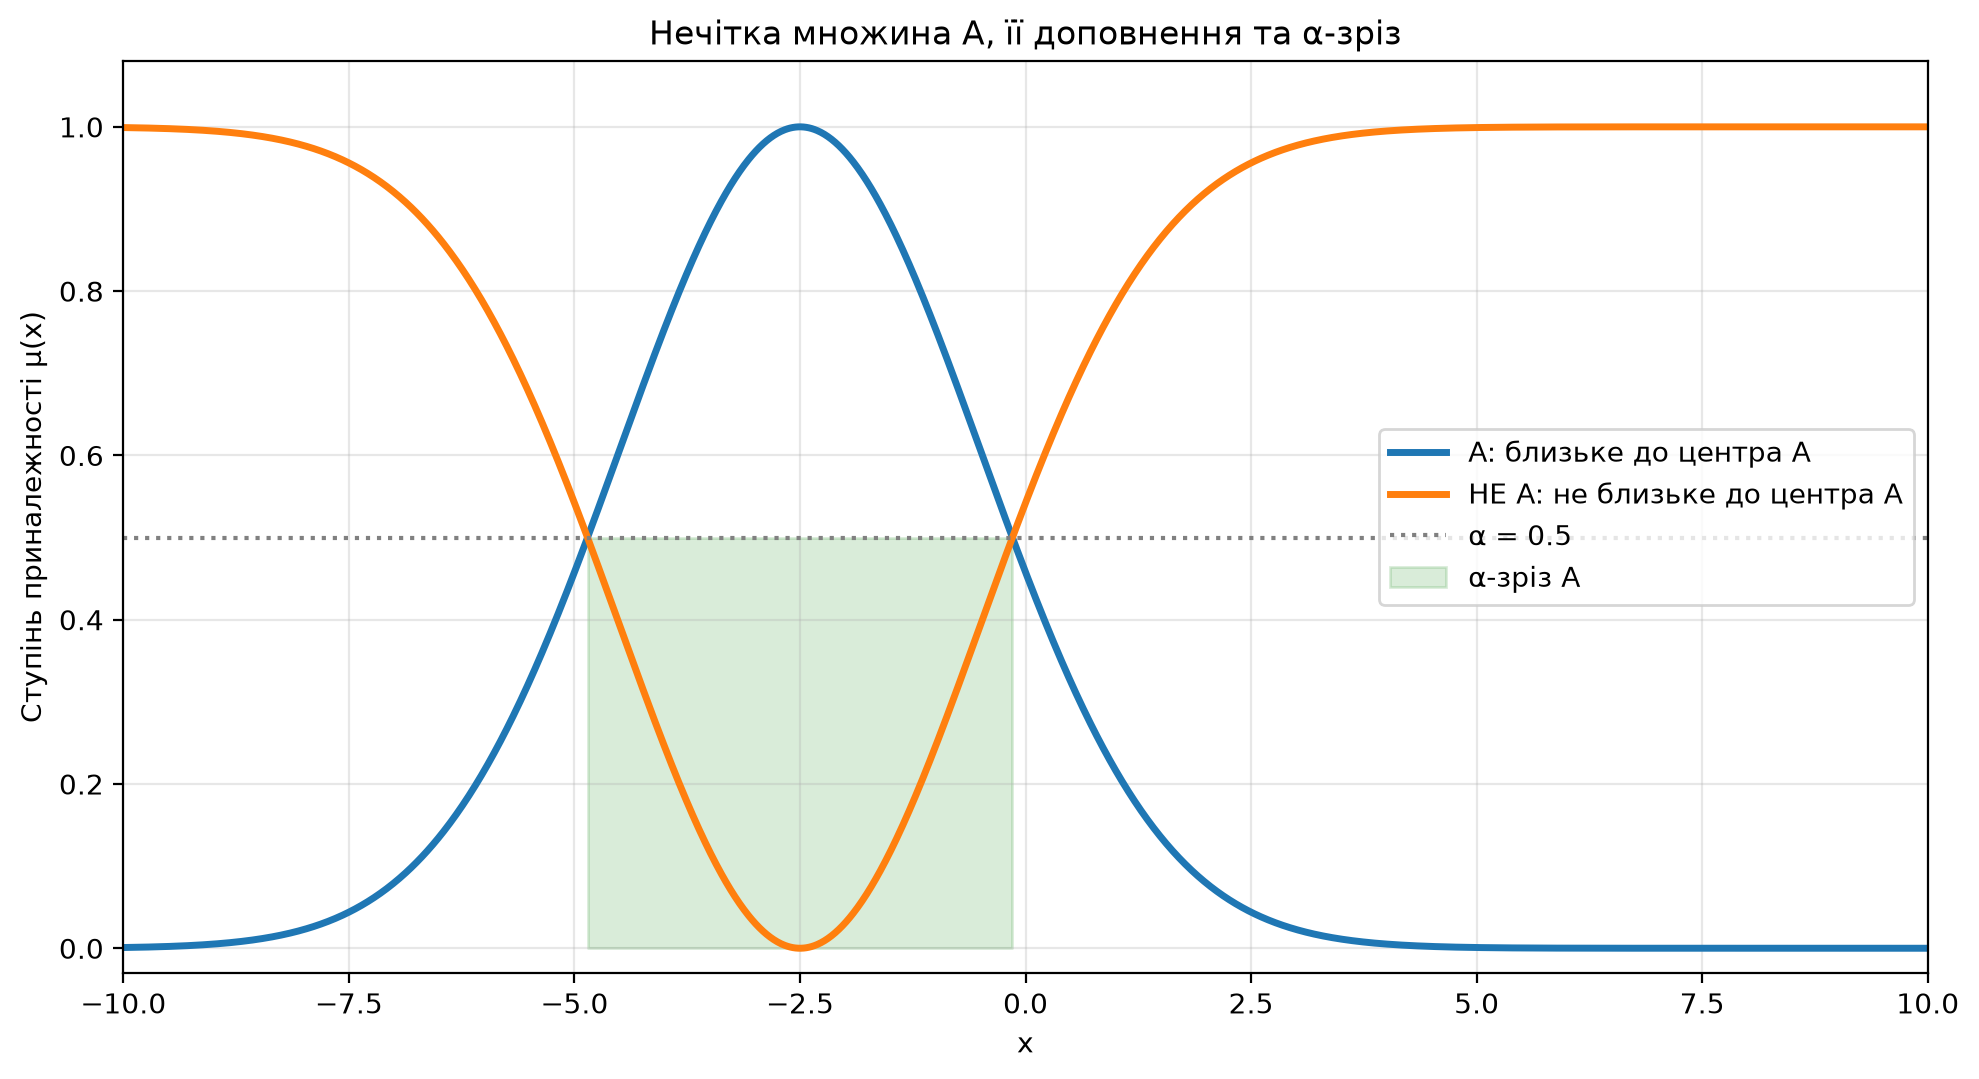
\includegraphics[width=\textwidth,height=0.42\textheight,keepaspectratio]{../src/figures/09_complement_alpha.png}
  \caption{Множина \(A\), її доповнення та \(\alpha\)-зріз}
  \label{fig:complement}
\end{figure}

\noindent
\textbf{Спостереження:}
максимальна похибка рівності \(\mu_A(x)+\mu_{\overline A}(x)=1\) становить
0, отже властивість доповнення виконується в усіх точках. Точки перетину
кривих мають ступінь приналежності 0{,}5. Для \(\alpha=0{,}5\) отримано
наближений зріз \([-4{,}84;-0{,}16]\).

\section{Висновки}

У лабораторній роботі сформовано нечіткі множини за допомогою трикутної,
трапецієподібної, простої та двосторонньої гаусових, узагальненої
дзвоноподібної, сигмоїдальних і поліноміальних функцій приналежності.
Встановлено, що параметри центрів переміщують криві вздовж універсуму,
параметри ширини змінюють область часткової приналежності, а коефіцієнти
нахилу та крутизни визначають різкість переходів.

Для двох гаусових множин виконано перетин та об'єднання в мінімаксній і
імовірнісній інтерпретаціях. Мінімаксні оператори поточково вибирають менше
або більше початкове значення. Імовірнісний добуток виявився не більшим за
мінімаксне перетинання, а алгебраїчна сума --- не меншою за мінімаксне
об'єднання. Також побудовано доповнення множини \(A\) і підтверджено
рівність \(\mu_A+\mu_{\overline A}=1\) з нульовою числовою похибкою. Усі
17 розрахованих масивів мають однакову довжину та значення в межах
\([0;1]\); програмна самоперевірка завершилася успішно.

\appendix
\section*{Відповіді на контрольні запитання}

\begin{enumerate}[leftmargin=*,itemsep=0.35em]
  \item Що таке нечітка множина і чим вона відрізняється від класичної
    (чіткої) множини?\\
    Нечітка множина допускає довільний ступінь приналежності з \([0;1]\),
    тоді як у чіткій множині можливі лише значення 0 або 1.
  \item Яке основне призначення функції приналежності в нечіткій множині?
    \\
    Вона чисельно задає ступінь відповідності кожного елемента поняттю,
    яке описує нечітка множина.
  \item У якому діапазоні приймають значення функції приналежності?
    \\
    У замкненому інтервалі \([0;1]\).
  \item Чим відрізняється повна належність елемента множині від часткової?
    \\
    Повній належності відповідає \(\mu(x)=1\), частковій ---
    \(0<\mu(x)<1\).
  \item Наведіть приклади реальних задач, де доцільно використовувати нечіткі
    множини.\\
    Керування кліматом, оцінювання ризику, медична діагностика, кредитний
    скоринг та системи підтримки прийняття рішень.
  \item Що таке універсальна множина у теорії нечітких множин?
    \\
    Це повна множина допустимих значень змінної, на якій визначено функцію
    приналежності.
  \item Які типові форми функцій приналежності застосовуються на практиці?
    \\
    Трикутні, трапецієподібні, гаусові, дзвоноподібні, сигмоїдальні та
    поліноміальні S-, Z- і PI-функції та інші.
  \item Яка різниця між трикутною та трапецієподібною функціями
    приналежності?\\
    Трикутна функція має одну вершину зазвичай зі значенням 1, а
    трапецієподібна --- інтервал повної приналежності.
  \item Як інтерпретувати значення функції приналежності, наприклад
    $\mu(x)=0{,}7$?\\
    Елемент відповідає описуваному нечіткому поняттю зі ступенем 0{,}7; І що важливо: це
    не слід автоматично трактувати як імовірність події.
  \item Що таке $\alpha$-рівень ($\alpha$-зріз) нечіткої множини?
    \\
    Це чітка множина всіх \(x\), для яких \(\mu(x)\geq\alpha\).
  \item Як визначається комплементарна (доповняльна) нечітка множина?
    \\
    Стандартне доповнення задається як
    \(\mu_{\overline A}(x)=1-\mu_A(x)\).
  \item У чому полягає відмінність між операціями об'єднання та перетину в
    нечітких множинах?\\
    Перетин реалізує нечітке «І», а об'єднання --- нечітке «АБО». Конкретно у
    мінімаксній інтерпретації їм відповідають мінімум і максимум.
  \item Що таке нечітке відношення і як воно пов'язане з функціями
    приналежності?\\
    Це нечітка множина на декартовому добутку універсумів; її функція
    приналежності задає ступінь зв'язку між кортежами елементів.
  \item Як можна використовувати функції приналежності для прийняття рішень у
    нечіткій логіці?\\
    Вони перетворюють точні вхідні значення на лінгвістичні оцінки, над
    якими виконують нечіткі правила, агрегацію та дефазифікацію результату.
  \item У чому полягають основні переваги нечітких множин у порівнянні з
    класичною логікою?\\
    Вони природно описують невизначені й мовні поняття, допускають плавні
    межі класів та дають змогу будувати зрозумілі правила без точної
    математичної моделі об'єкта. Випадок, коли природа не є дуалістичною.
\end{enumerate}

\end{document}
